% chktex-file 3 chktex-file 12 chktex-file 18 chktex-file 36 chktex-file 40
\section*{Exercise 5.11.}

Use the model defined in Problem 4.12 to find the best linear predictors of the Wolfer sunspot numbers $X_{1 0 1}, \ldots, X_{1 0 5}$ (being careful to take into account the non-zero mean of the series). Assuming that the series is Gaussian, ind 95\% prediction bounds for each value. (The observed values of $X_{1 0 1}, \ldots, \, X_{1 0 5}$ are in fact 139, 111, 102, 66, 45.) How do the predicted values $P_{1 0 0} X_{1 0 0+h}$ and their mean squared errors behave for large $h$ ?


\subsection*{Solution}

We insert the numbers from problem 4.12 and the sample numbers in the algorithm:
\[ Y_t = X_t - \underbrace{46.93}_{= \mu} \]
\[ Y_{t}-1.317Y_{t-1}+.634\,Y_{t-2}=Z_{t},\qquad\{Z_{t}\}\sim\mathrm{WN}(0,289.3). \]
\begin{minted}{python}
    mu = 46.93
    phi = 1 - 1.317 * z + 0.634 * z**2
    theta = 1
    sigma = np.sqrt(289.3) # standard deviation
    X = np.array([
        0, 101, 82, 66, 35, 31, 7, 20, 92, 154, 125,
        85, 68, 38, 23, 10, 24, 83, 132, 131, 118,
        90, 67, 60, 47, 41, 21, 16, 6, 4, 7, 
        14, 34, 45, 43, 48, 42, 28, 10, 8, 2,
        0, 1, 5, 12, 14, 35, 46, 41, 30, 24,
        16, 7, 4, 2, 8, 17, 36, 50, 62, 67,
        71, 48, 28, 8, 13, 57, 122, 138, 103, 86,
        63, 37, 24, 11, 15, 40, 62, 98, 124, 96,
        66, 64, 54, 39, 21, 7, 4, 23, 55, 94,
        96, 77, 59, 44, 47, 30, 16, 7, 37, 74
    ])
    Y = X - mu
    plt.plot(Y)
\end{minted}

\begin{figure}[H]
    \centering
    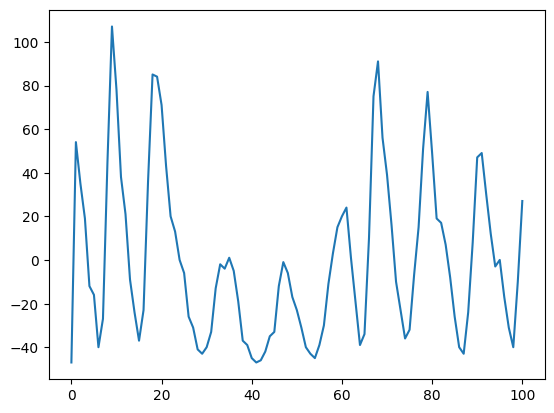
\includegraphics[width=0.65\textwidth]{../pictures/image1.png}
\end{figure}

Then, using the same algorithm for the previous method,
\begin{minted}{python}
    mu_n = h_step_prediction(phi,theta,sigma,Y,5)[101:].astype(float)
    sigma_n = np.sqrt(np.array([mean_square_error(i) for i in range(1,6)]).astype(float))
\end{minted}
to obtain the following results we recenter again to the original expected value
\[ P_n X_{n+h} = P_n Y_{n+h} + \mu \]
\begin{table}[H]\centering
    \begin{tabular}{l|ll}
    $h$ & $P_{100} X_{100+h}$ & $\sigma_n^2(h)$ \\ \hline
    1 & 88.87681    & 289.3 \\
    2 & 85.01156877 & 791.0876677  \\
    3 & 70.48914853 & 1141.45196582 \\
    4 & 53.81368401 & 1250.6469773 \\
    5 & 41.05931168 & 1254.23782416 \\       
    \end{tabular}
\end{table}

Also, it seems that after some iterations, $P_n X_{n+h}$ converges to $0$ and $\sigma_n^2$ converges to $1380.67330749$ when $h$ gets larger:

\begin{figure}[H]
    \centering
    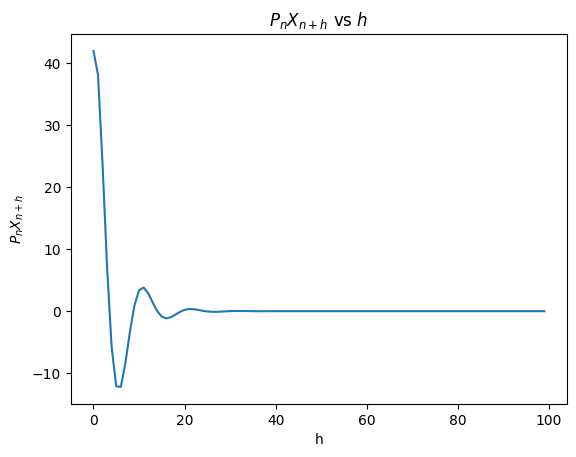
\includegraphics[width=0.45\textwidth]{../pictures/image2.png}
    \hfill
    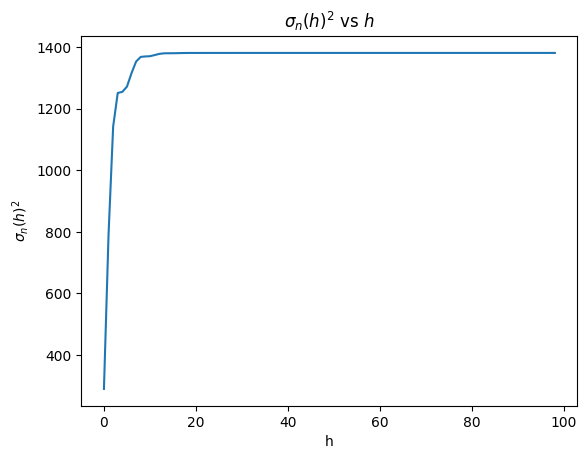
\includegraphics[width=0.45\textwidth]{../pictures/image3.png}
\end{figure}

Finally, the bounds for the confidence interval are:

\begin{table}[H]\centering
    \begin{tabular}{l|ll}
    $h$ & $P_n X_{n+h}+\Phi_{0.025}$ & $P_n X_{n+h}+\Phi_{0.975}$ \\ \hline
    1 & 55.540 & 122.213 \\
    2 & 29.885 & 140.138 \\
    3 & 4.271 & 136.707 \\
    4 & -15.499 & 123.127 \\
    5 & -28.353 & 110.472 \\
    \end{tabular}
\end{table}